\chapter{Neutrinos und Neutrinomischung in verschiedenen Basen}
\label{chap:neutrinobasen}

\section{Flavourbasis} %\cite[Kap. 2.1]{oberauer}
\label{subsec:flavourbasis}
Voraussetzung für die Neutrinooszillationen ist aber, dass Masseneigenzustände $\nu_i$ als Lösungen der Diracgleichung mit den Masseneigenwerten $m_i \neq 0 (i = 1, 2, 3)$ existieren.
Diese Masseneigenzustände bestimmen die Propagation des Neutrinos im Vakuum und müssen nicht zwangsläufig identisch zu den Flavoureigenzuständen sein.
Hier betrachten wir die Flavoureigenzustände $\nu_\alpha (\alpha = e, \mu, \tau)$ als Superposition der Masseneigenzustände mit
\begin{equation}
    \nu_\alpha = \sum_i U_{\alpha i} \nu^{(h_i)}_i \,,
    \label{eq:flavourbasis}
\end{equation}
wobei $U_{\alpha i}$ die unitäre Mischungsmatrix zwischen Massenbasis und Flavourbasis darstellt \cite[Kap. 2.1]{oberauer}.
Das Superskript $(h_i) = \pm 1$ beschreibt dabei die Helizität des Eigenzustands.


\section{Supernovae}

Im Inneren eines Sterns, der massiver als zehn unserer Sonnenmassen ist und sich dem Ende seines Lebens zuneigt, sind die Elemente nach absteigender Masse geschichtet.
Der Kern des Sterns, bestehend aus Eisen, Elektronen, Positronen, Photonen und vereinzelten Nukleonen, ist umgeben von Schichten aus Silizium, Sauerstoff, Kohlenstoff, Helium und Wasserstoff.
Je mehr Eisen der Stern jedoch fusioniert, desto weniger Material bleibt ihm zur weiteren Kernfusion übrig.
Zu diesem Zeitpunkt des Lebens des Sterns wird das Gleichgewicht zum nach innen wirkenden Gravitationsdruck durch den Strahlungsdruck der Elektronen nach außen aufrechterhalten. 
Doch dieses Gleichgewicht ist auf Dauer nicht stabil.

Die Elektronen und Protonen im Kern des Stern kombinieren im Prozess des Elektroneneinfangs zu einem Neutron und einem Elektronneutrino $e^- + p \rightarrow n + \nu_e$ \cite{supernovaepaper}.
So sinkt der Elektronendruck immer weiter, bis der Kern instabil wird und stürzt in sich zusammen, er kollabiert.
Die Kollapsgeschwindigkeit übersteigt dabei die Schallgeschwindigkeit im stellaren Medium, es erreicht also keine Information des zusammenbrechenden inneren Kerns den nachfolgenden äußeren Kern.
Mit einer anfänglichen Dichte von $10^9$ bis $10^{10} \, \si{\gram \per \centi\cubic\meter}$ erreicht er schnell Dichten, die in Nuklei, also Atomkernen, typisch sind.
In Zuge dessen durchläuft ändert sich die Zusammensetzung im Kern.
Nun besteht er nur noch aus Protonen und Neutronen.
Als Fermionen können nach dem Pauliverbot niemals zwei Fermionen im exakt gleichen Zustand existieren.
Zusätzlich zu diesem Verbot kommt hinzu, dass Protonen sich aufgrund ihrer gleichen Ladung abstoßen.

Je dichter der Kern beim Kollaps also wird, desto drastischer erhöht sich der Druck nach außen, bis der Kern im \textit{Rebound} von sich selber abprallt und eine Schockwelle erzeugt, die nach außen durch den Stern propagiert.
Dabei verliert die Schockwelle durch das Aufbrechen des einfallenden Sternmaterials Energie.
Zusammen mit der Energie, die durch Elektronneutrinos, die beim Elektroneneinfang mit den im Kern freiwerdenden Protonen entstehen, verloren geht, wird die Schockwelle im Kern verzögert, bevor sie vollends nach außen propagiert.
Der Kern des sterbenden Sterns mit seinem vergleichsweise kühlen Inneren und heißen, Neutrinos aller Flavours abstrahlenden Mantel wird nun als Protoneutronenstern bezeichnet.
Die im, auch Neutrinosphäre genannten Mantel freiwerdenden Neutrinos entstehen in so großer Zahl, dass eine Leistung von mehr als $10^{45} \,\si{\watt}$ frei wird, die die verzögerte Schockwelle wiederbelebt.
So explodiert der Stern in einer spektakulären Explosion, die wir als Supernova bezeichnen.

\section{Materiebasis} %\cite{päspaper}
\label{subsec:materiebasis}

Dabei wird ein großer Teil der Supernovaenergie durch Neutrinos propagiert.
Ist es diesen nun möglich, bei der Propagation durch das Supernovamedium über den Zerfall $\tilde{\nu}^{(h_i)}_i (p_i) \rightarrow \tilde{\nu}^{(h_j)}_j (p_j) + J(q)$
Energie in Form von Majoronen $J$ mit Impuls $q$ abzustrahlen, kann sich, je nach Kopplungsstärke zwischen Neutrino und Majoron, das Energiespektrum der Supernova verändern.
Diese Stöße wirken sich auf das Oszillations- und Propagationsverhalten der Neutrinos aus und können mithilfe der Materiebasis beschrieben werden.

Drücken wir dabei das linkshändige vierkomponentige Feld $\nu_L$ in chiraler Darstellung der Gammamatrizen über ein zweikomponentiges Feld $\phi$ mit $\nu^T_L = (\phi, 0)^T$ aus, 
näheres dazu findet sich in \cite{komponentendinger}, lässt sich der Lagrangian in der Materiebasis als
\begin{equation}
    \mathcal{L}_\text{tot} = \mathcal{L}_0 + \mathcal{L}_\text{med} + \mathcal{L}_\text{int}
    \label{eq:materielagrange}
\end{equation}
mit
\begin{align*}
    \mathcal{L}_0          &=   i \sum_i \left[\phi^\dagger_i \left(\partial_t - \vec{\sigma} \times \nabla \right) \phi_i - \frac{m_i}{2} \left(\phi^T_i \sigma_2 \phi - \phi^\dagger_i \sigma_2 \phi^*_i\right) \right] \,,\\
    \mathcal{L}_\text{med} &= - \sum_{i j} \phi^\dagger_i V_{i j} \phi_j  \,,\\
    \mathcal{L}_\text{int} &= - J \sum_{i j} g^M_{i j} \left( \phi^T_i \sigma_2 \phi_j + \phi^\dagger_i \sigma_2 \phi^*_j \right)
\end{align*}
schreiben \cite{päspaper}.
Dabei beschreibt der freie Lagrangian $\mathcal{L}_0$ die Propagation im Vakuum, $\mathcal{L}_\text{med}$ die in der Potentialmatrix $V$ berücksichtigten Effekte von Materie und $\mathcal{L}_\text{int}$
beschreibt Wechselwirkungen zwischen Neutrinos und Majoronen.
Die Kopplungsstärke zwischen Majoronen und Neutrinos der Massenbasis ist dabei in $g^M_{i j}$ zusammengefasst, $\vec{\sigma} = (\sigma_1, \sigma_2, \sigma_3)$ denotiert den Vektor der in \eqref{eq:paulimatrizen} zu findenden Paulimatrizen
und $m_i$ den Masseneigenwert des jeweiligen Neutrinos in der Massenbasis.
Wir berücksichtigen hier nur die einfachste Art der Majoronmodelle, also nehmen wir eine Proportionalität zwischen Kopplungs- und Massenmatrix $g^M_{i j} \propto m_{i j}$ an.

Für gewöhnlich würden wir hier, um die Eigenzustände des bereits erwähnten Zerfalls $\tilde{\nu}^{(h_i)}_i (p_i) \rightarrow \tilde{\nu}^{(h_j)}_j (p_j) + J(q)$ zu bestimmen, 
die aus $\mathcal{L}_\text{tot}$ resultierenden Feldgleichungen 
\begin{equation}
    i \left(\partial_t - \vec{\sigma} \times \nabla \right) \phi_i + i m_i \sigma_2 \phi^*_i - \sum^3_j V_{i j} \phi_j = 0 \,,
\end{equation}
wie in \cite{komponentendinger} gezeigt, mithilfe von Planarwellenspinoren definiter Helizität lösen, 
allerdings stimmen die so erhaltenden Lösungen mit den aus der Diagonalisierung der Mikheyev-Smirnov-Wolfenstein-Gleichung folgenden Lösungen überein.
Sie beschreibt die Zeitentwicklung schwacher Eigenzustände und die Mischung zwischen diesen und den Energieeeigenzuständen durch
\begin{equation}
    i \partial_t \nu^{(h)}_i = \left(H^\text{rel}_{i j} + U_{i \alpha} V_{\alpha \beta} U^\dagger_{\beta j}\right) \nu^{(h)}_j \,.
    \label{eq:MSW-gleichung}
\end{equation}
Aufgrund der geringen Massen und hohen Energien der Neutrinos, bei denen auch Energie- und Materieeigenzustände übereinstimmen, betrachten wir den hochrelativistischen Limes des Hamiltonians $H^\text{rel}_{i j} \approx \left(p + \frac{m^2_i}{2 p}\right) \delta_{ij}$ mit dem Kronecker-$\delta$
\begin{equation}
    \delta_{ij} = \begin{cases}
                    1, \quad i=j \\
                    0, \quad \text{sonst} \,.
                  \end{cases}
                  \label{eq:kronecker}
\end{equation}
$V$ ist dabei die diagonale Potentialmatrix der schwachen Basis, also
\begin{equation}
    V = \left( \begin{array}{c c c}
        V_C + V_N   &   0     &     0   \\ 
        0           &   V_N   &     0   \\ 
        0           &   0     &     V_N  \\
        \end{array}\right) \,,
\end{equation}
wobei $V_C = \sqrt{2} h G_F n_B (Y_\text{e}) + Y_{\nu_\text{e}}$ das von geladenen Strömen, also schwachen Wechselwirkungen, bei denen ein $W^+$- oder $W-$- Boson ausgetauscht wird erzeugte und 
$V_N = \sqrt{2} h G_F n_B \left(-\frac{1}{2} Y_N + Y_{\nu_\text{e}}\right)$ das durch ungeladene Ströme, also nur unter Austausch von neutralen $Z$-Bosonen stattfindende schwache Wechselwirkungen erzeugte Potential.
Mit der Baryonendichte $n_B$ des betrachteten Mediums gilt für ein beliebiges Teilchen $i$ mit korrespondierendem Antiteilchen $\bar{i}$ $Y_i = \frac{n_i - n_{\bar{i}}}{n_B}$.

Aus der Diagonalisierung der rechten Seite der MSW-Gleichung folgen die Materieeigenzustände
\begin{equation}
    \tilde{\nu}^{(h_i)}_i = \sum_i \tilde{U}_{i j} \nu^{(h_j)}_j \,.
    \label{eq:materiebasis}
\end{equation} 
Ähnlich wie die Flavoureigenzustände lassen sie sich als Superposition der Masseneigenzustände beschreiben.
Sie unterscheiden sich lediglich in der Mischungsmatrix $\tilde{U}$.

Hier können wir die in \autoref{subsec:flavourbasis} auftretende Mischungsmatrix $U$ als
\begin{equation}
    U = U_{2 3} \, U_{1 3} \, U_{1 2} \, U_0
    \label{eq:kopplungflavour}
\end{equation}
parametrisieren.
Bei den Matrizen $U_{i j}$ handelt es sich dabei um Rotationsmatrizen, die in der $i j$-Ebene eine Rotation um den Winkel $\theta_{i j}$ durchführen.
Die in \autoref{sec:neutrinomasse} behandelte mögliche CP-Verletzung findet sich als Phase in der Matrix $U_0$ wieder.

Wie in \cite{theta13} festgestellt ist $\theta_{1 3}$ nicht, wie lange Zeit angenommen, null.
Nach aktuellen Daten der Particle Data Group gilt $\sin^2 \left(\theta_{1 3} \right) = \num{2.20 +- 0.07} \cdot 10^{-2}$ \cite{neutrinospdg}, hier wird $\theta_{1 3}$ dennoch auf null gesetzt.

Damit vereinfacht sich die Mischungsmatrix zu $U = U_{2 3} \, U_{1 2} \, U_0$.
Jetzt können wir $\theta_{1 2}$ als solaren Mischungswinkel $\theta_\odot$ und $\theta_{2 3}$ als atmosphärischen Mischungswinkel $\theta_\text{atm}$ identifizieren.
Da zusätzlich, vor allem für leichte Neutrinos in der Nähe der Neutrinosphäre der Supernova, $|V_{\alpha \alpha}| \gg \frac{m^2_i}{2 p}$ für alle Elemente der Potentialmatrix gilt, unterscheiden sich die Materieeigenzustände nur um eine
beliebige Drehung $\theta'$ in der $\nu_\mu$ - $\nu_\tau$ Ebene von den Eigenzuständen der schwachen Basis.
Wir wählen $\theta' = -\theta_\text{2 3}$, um möglichst einfache Ausdrücke der Materieeigenzustände zu erhalten, wie sie in \autoref{tab:materieeigis} dargestellt sind.
\begin{table}[H]
    \centering
    \begin{tabular}{S S S}
      \toprule
    {Materieeigenzustände $\tilde{\nu}^{(h_i)}_i$} & {Schwache Eigenzustände $\nu_{\alpha'}$} & {Potential $V$} \\
      \midrule
       {$\tilde{\nu}^+_1$} & {$\bar{\nu}_e$}                                                        &  {$- (V_C + V_N)$} \\
       {$\tilde{\nu}^+_2$} & {$\bar{\nu}_{\mu'}  = c_{2 3} \bar{\nu}_\mu - s_{2 3} \bar{\nu}_\tau$} &  {$- V_N$} \\
       {$\tilde{\nu}^+_3$} & {$\bar{\nu}_{\tau'} = s_{2 3} \bar{\nu}_\mu + c_{2 3} \bar{\nu}_\tau$} &  {$- V_N$} \\
       {$\tilde{\nu}^-_1$} & {$\nu_{\mu'}        = c_{2 3} \nu_\mu       - s_{2 3} \nu_\tau$}       &  {$V_N$} \\
       {$\tilde{\nu}^-_2$} & {$\nu_{\tau'}       = s_{2 3} \nu_\mu       + c_{2 3} \nu_\tau$}       &  {$V_N$} \\
       {$\tilde{\nu}^-_3$} & {$\nu_e$}                                                              &  {$V_C + V_N$} \\
    \bottomrule
    \end{tabular}
    \caption{Materieeigenzustände $\tilde{\nu}^\pm_i$ positiver und negativer Helizität im Limes $|V_{\alpha \alpha}| \gg \frac{m^2_i}{2 p}$ als Rotation der schwachen Eigenzustände. Die Eigenzustände sind dabei so
            angeordnet, dass das Potential in der Tabelle nach unten hin ansteigt. Es gilt $c_{2 3} = \cos(\theta_{2 3})$ und $s_{2 3} = \sin(\theta_{2 3})$.}
    \label{tab:materieeigis}
\end{table}

Genauso lassen sich auch die Kopplungsmatrixelemente $\tilde{g}_{i j}$ der Materiebasis als Rotation der Elemente der schwachen Basis identifizieren.
In den hier betrachteten Modellen ist die schwache Kopplungsmatrix diagonal, es gilt also
\begin{equation}
    g^W = \left( \begin{array}{c c c}
        g_1         &   0     &     0   \\ 
        0           &   g_2   &     0   \\ 
        0           &   0     &     g_3  \\
    \end{array}\right) \,.
    \label{eq:schwachekopplung}
\end{equation}

Damit ist also
\begin{equation}
    g_{\alpha' \beta'} \equiv \ \tilde{g}_{i j} = U(-\theta_{2 3}) \, g^W_{\alpha \beta} \, U^T(-\theta_{2 3}) = U_{1 2} \, U^*_0 \, g^M_{i j} \, U^\dagger_0 \, U_{1 2} \,,
\end{equation}
wenn wir zusätzlich benutzen, dass die schwache Kopplungsmatrix und die der Massenbasis über $g^W = U \, g^M \, U^T$ verknüpft sind, oder explizit
\begin{align}
    \tilde{g} &= \left( \begin{array}{c c c}
        g_{ee}                  &   g_{e \mu'}          &     g_{e \tau'}       \\ 
        g_{e \mu'}              &   g_{\mu' \mu'}       &     g_{\tau' \mu'}    \\ 
        g_{e \tau'}             &   g_{\tau' \mu'}      &     g_{\tau \tau}     \\
    \end{array}\right) \nonumber\\
    &= \left( \begin{array}{c c c}
        g_1 \cos^2 \theta_\odot + g_2 sin^2 \theta_\odot \mathrm{e}^{-2 i \delta}                   &   \frac{1}{2} \left(-g_1 + g_2 \mathrm{e}^{-2 i \delta}\right) \sin(2 \theta_\odot)       &     0   \\ 
        \frac{1}{2} \left(-g_1 + g_2 \mathrm{e}^{-2 i \delta}\right) \sin(2 \theta_\odot)           &   g_1 sin^2 \theta_\odot + g_2 \cos^2 \theta_\odot\mathrm{e}^{-2 i \delta}                &     0   \\ 
        0                                                                                           &   0                                                                                       &     g_3  \\
    \end{array}\right)
    \label{eq:materiekoppmat}
\end{align}
mit der CP-verletzenden Phase $\delta$ \cite{päspaper}.
Die Kopplungsparameter $g_2$ und $g_3$ lassen sich dabei in Abhängigkeit von $g_1$ und $m_1$, also der Masse des ersten Masseneigenzustands, ausdrücken als
\begin{align}
    g_2 = g_1 \sqrt{1 + \frac{\Delta m^2_\odot}{m^2_1}}\,, && g_3 = g_1 \sqrt{1 + \frac{\Delta m^2_\odot + \Delta m^2_\text{atm}}{m^2_1}} \,,
    \label{eq:g2g3}
\end{align}
wobei wir die Definitionen $\Delta m^2_{1 2} = m^2_2 - m^2_1 = \Delta m^2_\odot$ und $\Delta m^2_{23} = m^2_3 - m^2_2 = \Delta m^2_\text{atm}$ benutzen.
So ist also ein Zusammenhang der Kopplungsmatrizen aller drei Basen hergestellt, der im folgenden genutzt werden kann, um die Einschränkungen auf die Kopplungsstärken deutlich zu machen.


\section{Einschränkung der Kopplungsparameter durch Supernovae}

Im Folgenden betrachten wir einige der Argumente, die genutzt werden können, um die Kopplungsparameter zwischen Majoronen und Neutrinos einzuschränken, näher.
Konkret gehen wir auf die Einschränkungen durch Neutrinospektren ein, die es uns ermöglichen, die Kopplungsparameter $g_1$ und $g_2$ einzuschränken, und die Einschränkungen aus der Majoronenluminosität ein,
die uns eine Ausschlussregion für $|\tilde{g}_{i j}|$ liefert.
Zusätzlich wird kurz das aktuelle Limit auf die Neutrinomasse $m_1$ diskutiert.

\subsection{Grenzen durch Neutrinospektren}
\label{subsec:spektrengrenzen}

Durch Majoronen induzierte Flavourübergänge der Neutrinos der Form $\tilde{\nu}^\pm_i \rightarrow \tilde{\nu}^\mp_j + J$ können das Energiespektrum der einzelnen Neutrinogenerationen merklich verschieben. 
Dabei muss jedoch beachtet werden, dass die Wirkungsquerschnitte der unterschiedlichen Neutrinos innerhalb einer typischen Supernova nicht übereinstimmen.
Diese Diskrepanz stammt daher, dass $\nu_\mu$ und $\nu_\tau$ nur über neutrale Ströme mit dem Supernovamedium interagieren können.
Innerhalb von Supernovae verhalten $\nu_\mu$ und $\nu_\tau$ sich also nahezu gleich.
Elektronneutrinos $\nu_e$ können dagegen nicht nur über neutrale, sondern auch über geladene Ströme mit dem Medium wechselwirken.
So können sie unter Abstrahlung eines $W$-Bosons mit den im Überfluss vorhandenen Elektronen interagieren, während Wechselwirkungen von $\nu_\mu$ und $\nu_\tau$ mit der Materie in den dichteren Regionen des sterbenden Sterns kaum zustande kommen.
Es entsteht also ein Spektrum niedrigerer Temperaturen für $\nu_e$ und höherer Temperaturen für $\nu_\mu$ und $\nu_\tau$, dass durch Neutrinozerfälle verzerrt werden kann.
Berücksichtigen wir nun zusätzlich zur Zerfallswahrscheinlichkeit $N_\text{decay}$ außerdem die Oszillationswahrscheinlichkeit $N_\text{osc}$ der Neutrinos nach dem Verlassen seiner Energiesphäre mit Radius $R_{E, \tilde{\nu}^\pm_i}$, 
bis sie hier auf der Erde ankommen, lässt sich die effektive Wahrscheinlichkeit, dass ein Neutrino mit seinem ursprünglichen Flavour die Erde erreicht, als
\begin{equation}
    N = N_\text{decay} \cdot N_\text{osc}
    \label{eq:survivalprob}
\end{equation}
schreiben \cite{supernovaboundsdasandere}.

Die Zerfallswahrscheinlichkeit ist dabei gegeben durch
\begin{equation}
    N_\text{decay}(\tilde{\nu}^\pm) \cong \exp \left(- \int^\infty_{R_{E, \tilde{\nu}^\pm_i}} \mathrm{d}r \, \sum_j \Gamma(\tilde{\nu}^\pm_i \rightarrow \tilde{\nu}^\mp_j + J) \right) \,.
    \label{eq:zerfallswkeit}
\end{equation}
In relativistischer Näherung, die wir hier bereits zur Bestimmung der Materieeigenzustände verwendet haben, lässt sich die Zerfallsrate $\Gamma(\tilde{\nu}^\pm_i \rightarrow \tilde{\nu}^\mp_j + J)$ durch
\begin{equation}
    \Gamma(\tilde{\nu}^\pm_i \rightarrow \tilde{\nu}^\mp_j + J) = \frac{|\tilde{g}^2_{i j}|}{16 \pi} \left(V_i - V_f \right)
    \label{eq:zerfallsrate}
\end{equation}
ausdrücken, wobei $V_i - V_f$ die Potentialdifferenz zwischen Anfangs- und Endzustand beschreibt.

Die Oszillationswahrscheinlichkeit hängt stark von der gewählten Massendifferenz und dem Mischungswinkel zwischen den Neutrinos ab.
Wir fokussieren uns hier auf die LMA-MSW, also die Large-Mixing-Angle MSW-Lösung, die einen großen Mischungswinkel annimmt.
Wie in \cite{ueberlebenswkeit} genauer erläutert ergibt sich so eine Oszillationswahrscheinlichkeit von
\begin{equation}
    N_\text{osc} = 1 - \left[\sin^2\theta_\odot - \sin 2\theta_m \sin\left(2\theta_\odot - 2 \theta_m\right) \sin^2 \left(\frac{\pi d}{l_m}\right)\right] \,,
    \label{eq:osziwkeit}
\end{equation}
wobei
\begin{equation*}
    l_m = \frac{4 \pi E}{\Delta m^2_\odot} \frac{\sin2\theta_m}{\sin2\theta_\odot}
\end{equation*}
die Oszillationslänge und $\theta_m$ den Mischungswinkel der Neutrinos in Materie, die sie auf einer Distanz $d$ in der Erde bis zum Detektor durchdringen, beschreibt.
Durch die Näherung $\theta_{1 3} = 0$ gehen wir davon aus, dass es nur zu einer Mischung zwischen Elektron- und Myonneutrinos kommt, der Mischungswinkel $\theta_m$ lässt sich also mit $\theta_\odot$ identifizieren.
So lassen sich, wenn wir, wie in \cite{supernovaboundsdasandere} gezeigt, die entsprechenden, fehlenden Größen in \eqref{eq:osziwkeit} einsetzen, die Kopplungsparameter $g_1$ und $g_2$ auf einige $10^{-4}$ einschränken.

\subsection{Grenzen durch Majoronenluminosität}

Um die Grenzen auf die Kopplungsparameter $|g_{i j}|$ aus der Majoronenluminosität zu erhalten, betrachten wir das Neutrinosignal der Supernova SN$1987$A unter der Annahme, dass $\nu_e$ nur geringfügig mit den anderen Flavours mischt.
Unter dieser Annahme passt das beobachtete Neutrinosignal gut zu numerischen Berechnungen der totalen Bindungsenergien in einer Supernova und erlaubt es uns, eine Ausschlussregion von auf die Kopplungsparameter durch
\begin{equation}
    3 \cdot 10^{-7} < |g_{i j}| < 2 \cdot 10^{-5} %%%%%%%%%%%%%%% TEMP!!!! AKTUALISIERUNG MIT DEN NEUEN DATEN. PÄS BITTE ANTWORTE MIIIIIR
    \label{eq:gijlimit}
\end{equation}
festzulegen.

Lägen die Kopplungen in dem ausgeschlossenen Bereich, würden wir eine merkliche Unterdrückung der beobachteten Energie erwarten.
Für Werte $|g_{i j}| < 3 \cdot 10^{-7}$ wird die Kopplung zwischen Neutrinos und Majoronen so schwach, das kein merklicher Effekt auf das Supernovaspektrum entstehen würde. %%%% HIER SIND AUCH NOCH ALTE LIMITS!
Auf der anderen Seite wird die Kopplung für $|g_{i j}| > 2 \cdot 10^{-5}$ so stark, dass die Majoronen das Innere der Supernova nicht länger verlassen könnten. %%%% HIER SIND AUCH NOCH ALTE LIMITS!
So würden sie ebenfalls nicht zu einer Änderung des Energiespektrums beitragen.


\subsection{Neutrinomassengrenze aus KATRIN}
\label{subsec:KATRIN}

Das KATRIN-Experiment in Karlsruhe ist in der Lage, die Masse des Elektronneutrinos stark einzuschränken.
Dies ist möglich, indem das kontinuierliche Energiespektrum der Elektronen beim $\beta$-Zerfall genauestens untersucht wird, genauer genommen das Abknicken dieses Spektrums für die maximale Elektronenenergie.
Dieser Knick ist näher in \autoref{fig:elektronenspektrum} dargestellt.
\begin{figure}[H]
    \centering
    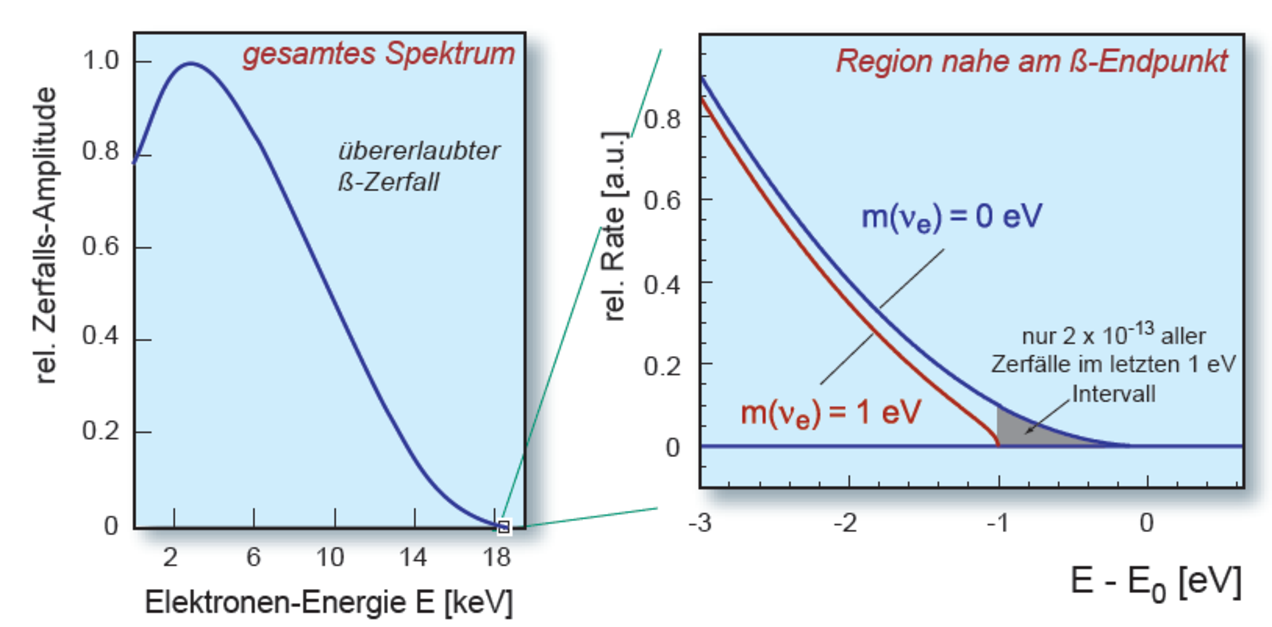
\includegraphics[width=.5\textwidth]{figures/Elektronenspektrum.pdf}
    \caption{Spektrum der Elektronen beim $\beta$-Zerfall. Die linke Kurve zeigt das gesamte Spektrum von der minimalen bis zur maximalen Energie, die das Elektron während des Zerfalls erhält. Rechts
            ist hochenergetische Ende der Kurve vergrößert dargestellt. Es wird ein Vergleich zwischen dem Kurvenverlauf unter der Annahme eines masselosen Neutrinos $m(\nu_e) = 0$ und dem Kurvenverlauf unter Freisetzung
            eines Elektronneutrinos mit einer Masse von $1 \si{\eV}$ hergestellt. Charakteristisch ist das Abknicken der Kurve für $m(\nu_e) \neq 0$. Dieses Abknicken stammt daher, dass das Elektron nicht länger
            die maximale Stoßenergie besitzen kann, sobald das Neutrino Masse besitzt \cite{elektronenspektrum}.}
    \label{fig:elektronenspektrum}
\end{figure}
Durch die Analyse der Position dieses Knicks konnte die Neutrinomasse Anfang $2022$ auf $m_1 < \SI{0.8}{\eV}$ \cite{KATRINneutrinogrenze} eingeschränkt werden.
Gemeinsam mit den in \autoref{subsec:spektrengrenzen} gefundenen Einschränkungen auf $g_1$ und damit auch auf $g_2$ lässt sich so das Fenster wählen, in dem die erstellten Plots relevant sind.




